\chapter{Attacks}
\label{chap:attacks}
A Pokémon deals damage in battle via two types of attacks.
``Fast'' attacks generate the energy required by powerful ``charged'' attacks.
Energy is preserved across substitution, but not across battles.
Every attack has a single type, which may or may not be a type of the attacker.
Attacks having a type in common with the attacker enjoy a 1.2x multiplier, the Same Type Attack Bonus (STAB).
A single attack usually has different stats for Raids/Max Battles (\autoref{sec:nx1})
  and Trainer Battles (\autoref{sec:3x3}).

As developed in \autoref{sec:dualtypes}, an attack's type effectiveness
  against a given opponent ranges from -3 to 2, inclusive.
See \autoref{sec:typemult} for the quantitative impact of type effectiveness.
Using \autoref{table:relations}, we assign each attacking type $A$ four values
  $R_{-2}\cdots{}R_1$, where $R_n$ is the number of types against which $A$ has a
  relation of $n$.
To calculate the number of typings $E_n$ against which $A$ has some effectiveness $n$
  using the following relations (\autoref{table:attackeff}):
\begin{align*}
  E_{-3} &= R_{-2}R_{-1}\\
  E_{-2} &= R_{-2}(R_0 + 1) + \binom{R_{-1}}{2}\\
  E_{-1} &= R_{-1}(R_0 + 1) + R_{-2}R_1\\
   E_{0} &= R_0 + \binom{R_0}{2} + R_{1}R_{-1}\\
   E_{1} &= R_{1}(R_0 + 1)\\
   E_{2} &= \binom{R_1}{2}\\
   ARA &= \frac{\sum_{i=-3}^{2} E_{i}i}{18}
\end{align*}
under the invariants:
\begin{align*}
    \sum_{i=-2}^{1} R_i &= 18\\
   \sum_{i=-3}^{2} E_i &= \binom{18}{2} + 18  = 171
\end{align*}
\begin{table}[ht]
  \centering
  \begin{tabular}{l r r r r|r r r r r r r}
    & \multicolumn{4}{c}{Type → Type} & \multicolumn{6}{c}{Type → Typing} & \\
    & \multicolumn{4}{c}{\downbracefill} & \multicolumn{6}{c}{\downbracefill} & \\
    $A$ & -2 & -1 & 0 & 1 & -3 & -2 & -1 & 0 & 1 & 2 & ARA \\
    \Midrule

\includegraphics[height=1em,keepaspectratio]{images/ground.png} & 1 & 2 & 10 & 5 & 2 & 12 & 27 & 65 & 55 & 10 & 1 \\

\includegraphics[height=1em,keepaspectratio]{images/rock.png} & 0 & 3 & 11 & 4 & 0 & 3 & 36 & 78 & 48 & 6 & 1 \\

\includegraphics[height=1em,keepaspectratio]{images/fairy.png} & 0 & 3 & 12 & 3 & 0 & 3 & 39 & 87 & 39 & 3 & 0 \\

\includegraphics[height=1em,keepaspectratio]{images/flying.png} & 0 & 3 & 12 & 3 & 0 & 3 & 39 & 87 & 39 & 3 & 0 \\

\includegraphics[height=1em,keepaspectratio]{images/fire.png} & 0 & 4 & 10 & 4 & 0 & 6 & 44 & 71 & 44 & 6 & 0 \\

\includegraphics[height=1em,keepaspectratio]{images/ice.png} & 0 & 4 & 10 & 4 & 0 & 6 & 44 & 71 & 44 & 6 & 0 \\

\includegraphics[height=1em,keepaspectratio]{images/water.png} & 0 & 3 & 12 & 3 & 0 & 3 & 39 & 87 & 39 & 3 & 0 \\

\includegraphics[height=1em,keepaspectratio]{images/ghost.png} & 1 & 1 & 14 & 2 & 1 & 15 & 17 & 107 & 30 & 1 & -1 \\

\includegraphics[height=1em,keepaspectratio]{images/steel.png} & 0 & 4 & 11 & 3 & 0 & 6 & 48 & 78 & 36 & 3 & -1 \\
    
\includegraphics[height=1em,keepaspectratio]{images/dark.png} & 0 & 3 & 13 & 2 & 0 & 3 & 43 & 96 & 28 & 1 & -1.0\textoverline{5} \\

\includegraphics[height=1em,keepaspectratio]{images/fighting.png} & 1 & 5 & 7 & 5 & 5 & 18 & 45 & 52 & 40 & 10 & -2 \\

\includegraphics[height=1em,keepaspectratio]{images/psychic.png} & 1 & 2 & 13 & 2 & 2 & 15 & 30 & 95 & 28 & 1 & -2 \\

\includegraphics[height=1em,keepaspectratio]{images/dragon.png} & 1 & 1 & 15 & 1 & 1 & 16 & 17 & 121 & 16 & 0 & -2 \\
    
\includegraphics[height=1em,keepaspectratio]{images/electric.png} & 1 & 3 & 12 & 2 & 3 & 11 & 41 & 89 & 26 & 1 & -2.\textoverline{4} \\

\includegraphics[height=1em,keepaspectratio]{images/bug.png} & 0 & 7 & 8 & 3 & 0 & 21 & 63 & 57 & 27 & 3 & -4 \\

\includegraphics[height=1em,keepaspectratio]{images/grass.png} & 0 & 7 & 8 & 3 & 0 & 21 & 63 & 57 & 27 & 3 & -4 \\

\includegraphics[height=1em,keepaspectratio]{images/poison.png} & 1 & 4 & 11 & 2 & 4 & 18 & 50 & 74 & 24 & 1 & -4 \\
    
\includegraphics[height=1em,keepaspectratio]{images/normal.png} & 1 & 2 & 15 & 0 & 2 & 17 & 34 & 118 & 0 & 0 & -4.\textoverline{1} \\
\end{tabular}
    \caption[Attack Type effectiveness summaries]{Attack Type effectiveness summaries (higher is better)}
    \label{table:attackeff}
\end{table}

\section{Fast Attacks}
Every Pokémon knows exactly one Fast Attack, which can be changed with a Fast TM
 (an Elite Fast TM allows the new attack to be chosen; it is otherwise random).
A fast attack is defined by its duration, its power, and the energy built up with each use (\autoref{table:fastattacks}).
Each Pokémon can store up to 100 units of energy, which is preserved across substitutions.
DPT and EPT are power and energy, respectively, normalized per turn.
If fast attack $A$ is stronger than fast attack $B$ in Nx1 mode, it will not be
  weaker than $B$ in 3x3 mode, and vice versa (i.e.\ partial ordering is maintained).
Furthermore, no fast attack's Nx1 power is less than its 3x3 power.
Incinerate is thus the most powerful fast attack in both modes.
It is also the only five turn attack, and the only one to hit 4 with both EPT and DPT\@.
Charm stands alone with a DPT of 5, with Razor Leaf coming in behind it at 4.5.
Lock On manages 5 EPT, with Psycho Cut, Poison Sting, Fairy Wind, Karate Chop,
  and Thunder Shock at 4.5.
Fast attacks counts are broken down by type in \autoref{table:attacktypes},
 and \autoref{chap:attackemployers} provides lists of Pokémon which can use each attack.
  \textbf{FIXME these are only training data, not valid for Nx1 battles!}
\input{out/fastattacks}
\input{out/attacktypes}

\begin{figure}[ht]
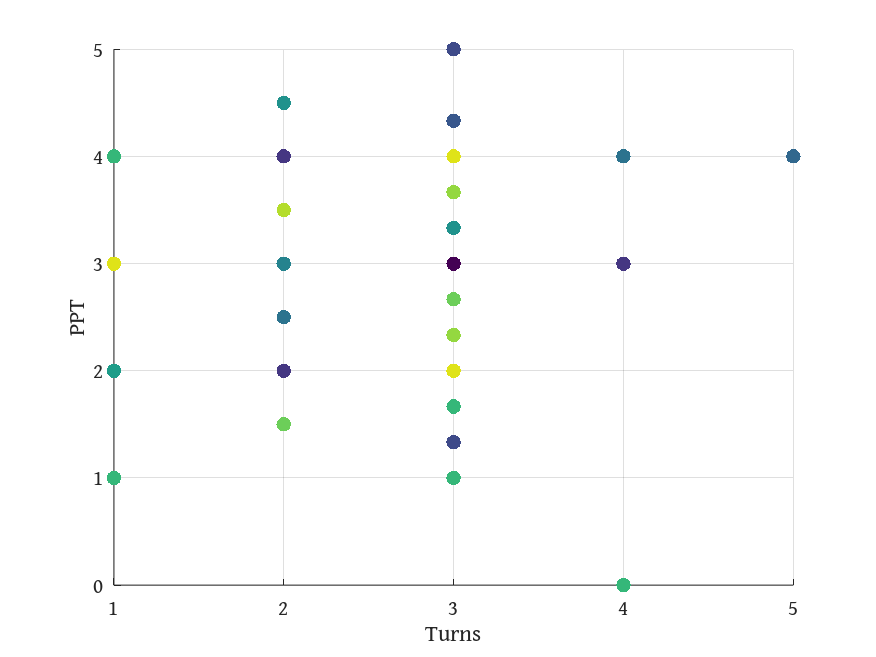
\includegraphics[keepaspectratio,width=\textwidth]{octave/pptvst.png}
\caption{PPT vs turns for fast attacks}
\label{fig:pptvst}
\end{figure}

\begin{figure}[hb]
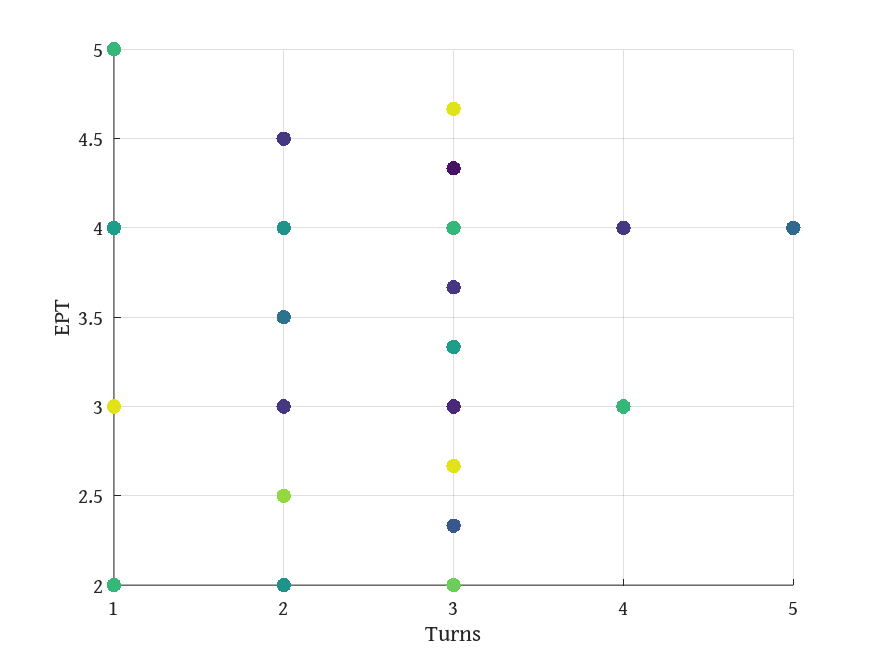
\includegraphics[keepaspectratio,width=\textwidth]{octave/eptvst.png}
\caption{EPT vs turns for fast attacks}
\label{fig:eptvst}
\end{figure}

\section{Charged Attacks}
\label{sec:charged}
Every Pokémon knows at least one Charged Attack, and most can be taught a second
  Charged Attack at a cost of Stardust and Candy\footnote{Applin, Combee,
  Cosmoem, Cosmog, Ditto, Gimmighoul, Toxel, Unown, and Wimpod are exceptions;
  none of them have a second charged attack to learn.}.
A Charged TM allows a charged attack to be changed (the Trainer can select
  which charged attack is replaced if the Pokémon knows two);
  an Elite Charged TM allows the Trainer to select the new charged attack.
A charged attack is defined by its power and the energy it consumes (\autoref{table:chargedattacks}).
Energy generated by the Fast Attack goes into a pool from which either Charged Attack can draw.
Unlike fast attacks, partial ordering is not generally preserved between Nx1 and 3x3 mode:
  Sunsteel Strike is the most powerful charged attack in Nx1, whereas Aeroblast tops
  the list in 3x3.
\input{out/chargedattacks}

In 3x3, each side starts with two Damage Shields.
The Trainer can deploy a Shield whenever the opponent prepares a charged attack,
   and the decision must be made before the particular attack is revealed.
Shields reduce the incoming damage to a single point, and each can be used only once.

\autoref{fig:dpevse} plots Power-per-Energy (PPE) against energy for charged attacks.
A higher PPE makes more efficient use of the energy built up by fast attacks.
A lower energy requires fewer fast attacks to build up its charge.
Note that many of the best PPEs do not require extreme energy; these make
 for excellent charged attacks.

\begin{figure}[ht]
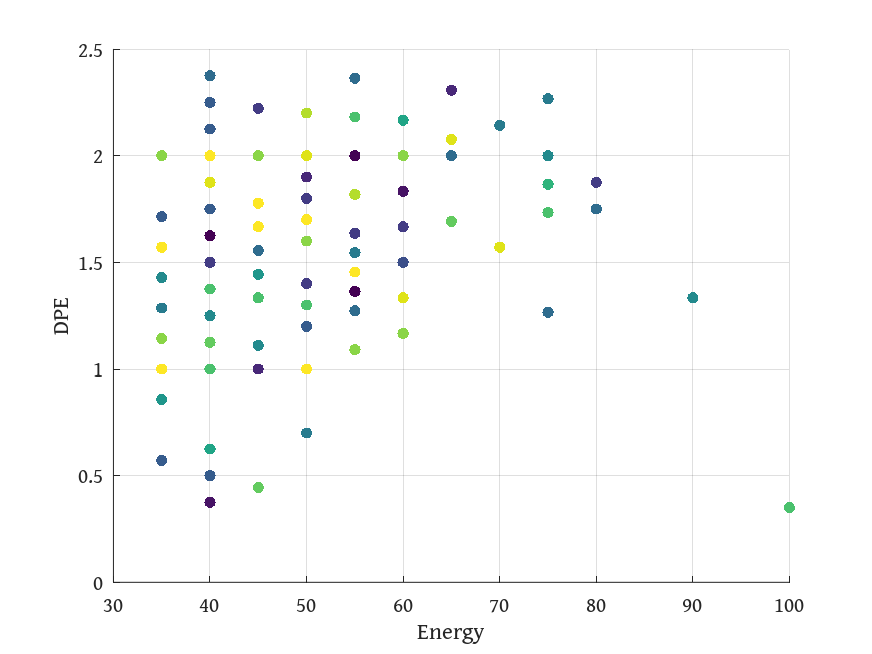
\includegraphics[keepaspectratio,width=\textwidth]{octave/dpevse.png}
\caption{PPE vs energy for charged attacks}
\label{fig:dpevse}
\end{figure}

\section{Buffs and debuffs}
\label{sec:buffs}
Certain charged attacks have a chance of semi-persistent effects on the
  attack or defense of the user or opponent.
These occur only in 3x3 battles, and are not affected by the use of a shield.
Several attacks (Ancient Power, Obstruct, Ominous Wind, Signal Beam, Silver
  Wind, Superpower, Tri Attack) can have multiple effects; in this case, any
  probabilistic check is done once for all effects---either all of them
  occur, or none of them do.
The effects apply only to the active Pokémon, and do not persist across substitution.
Stat changes stack, but the absolute value will not exceed four.
\begin{table}[ht]
  \centering
  \begin{tabular}{ll}
    Level & Change\\
    \Midrule
    -4 & -50\%\\
    -3 & -42.85\%\\
    -2 & -33.\textoverbar{3}\%\\
    -1 & -20\%\\
     1 &  25\%\\
     2 &  50\%\\
     3 &  75\%\\
     4 & 100\%\\
  \end{tabular}
  \caption{Mapping buff/debuff stages to effect}
\end{table}

\subsection{Adventure Effects}
\label{sec:effects}
\textbf{FIXME}

\section{Cover sets}
\label{sec:coversets}
It is a fine thing to have supremacy against any typing an opponent might bring onto the field.
With one fast and two charged attacks per Pokémon, a team of three can boast nine distinct attack types.
Can we achieve coverage of the defenders' typing with this limited repertoire?
Were we working against only monotyped Pokémon, nine types would be more than sufficient.
The smallest cover of all eighteen types is achieved with seven attacking types in
  ten different collections (\autoref{table:coversetsmono}).
Fighting is always necessary to gain advantage over Normal, and Ground is required for Electric.
No other types show up in all covering sets.
\begin{table}[ht]
\begin{centering}
  \begin{tabular}{c}
 Dark, Electric, Fighting, Flying, Ground, Ice, Poison\\
 Dark, Electric, Fighting, Flying, Ground, Ice, Steel\\
 Dark, Fairy, Fighting, Grass, Ground, Poison, Rock\\
 Dark, Fighting, Flying, Grass, Ground, Ice, Poison\\
 Dark, Fighting, Flying, Grass, Ground, Ice, Steel\\
 Electric, Fighting, Flying, Ghost, Ground, Ice, Poison\\
 Electric, Fighting, Flying, Ghost, Ground, Ice, Steel\\
 Fairy, Fighting, Ghost, Grass, Ground, Poison, Rock\\
 Fighting, Flying, Ghost, Grass, Ground, Ice, Poison\\
 Fighting, Flying, Ghost, Grass, Ground, Ice, Steel\\
  \end{tabular}
  \caption{Monotypes are minimally covered by 10 sets of 7}
  \label{table:coversetsmono}
\end{centering}
\end{table}

It's interesting to look at how these sets change if we ignore one target type.
Dropping Fairy, Normal, or Water results in coverage using only six attacking types,
  and can thus be handled with only charged attacks.
Dropping Dark, Fire, Ice, Poison, Psychic, Rock, or Steel doesn't change the solution space at all.
The remaining eight elisions merely enable more septuples (\autoref{table:partialcovers}).
\begin{table}[ht]
\begin{centering}
  \begin{tabular}{lrr|lrr}
    Ignored type & Cover size & Sets & Ignored type & Cover size & Sets\\
    \Midrule
    Bug & 7 & 30 & Dragon & 7 & 24\\
    Electric & 7 & 22 & Fairy & 6 & 4\\
    Fighting & 7 & 28 & Flying & 7 & 22\\
    Ghost & 7 & 16 & Grass & 7 & 12\\
    Ground & 7 & 24 & Normal & 6 & 2\\
    Water & 6 & 4 & & & \\
  \end{tabular}
  \caption{Partial covers are comparable in size to a full cover}
  \label{table:partialcovers}
\end{centering}
\end{table}

Of course, what we're really interested in covering is the full set
  of possible target typings, including all dualtypes.
Unfortunately, this requires no fewer than ten attacking types,
  which can be selected in nine different ways (\autoref{table:coversetsdual}).
\begin{table}[ht]
\begin{centering}
  \begin{tabular}{c}
 Dark, Fairy, Fighting, Fire, Grass, Ground, Poison, Rock, Steel, Water\\
 Dark, Fairy, Fighting, Fire, Grass, Ground, Ice, Poison, Rock, Steel\\
 Dark, Fairy, Fighting, Fire, Ghost, Grass, Ground, Poison, Rock, Water\\
 Dark, Fairy, Fighting, Fire, Ghost, Grass, Ground, Ice, Poison, Rock\\
 Dark, Fairy, Fighting, Fire, Flying, Grass, Ground, Rock, Steel, Water\\
 Dark, Fairy, Fighting, Fire, Flying, Grass, Ground, Ice, Rock, Steel\\
 Dark, Electric, Fairy, Fighting, Fire, Flying, Grass, Ground, Ice, Steel\\
 Bug, Dark, Fairy, Fighting, Fire, Grass, Ground, Rock, Steel, Water\\
 Bug, Dark, Fairy, Fighting, Fire, Grass, Ground, Ice, Rock, Steel\\
  \end{tabular}
  \caption{Full typing is minimally covered by 9 sets of 10}
  \label{table:coversetsdual}
\end{centering}
\end{table}

Even assuming unlimited substitution, this demonstrates the
  impossibility of assembling a team which can effectively
  hit every possible opposing Pokémon with some attack.
However, \autoref{sec:typeleagues} explores situations where typing is restricted.
In such cases, the minimum set concept is extremely powerful.

\section{Relative strength of fast and charged attacks}
\label{sec:fastvchaged}
It's sometimes useful to delay use of a charged attack, but is it ever wise to forgo
  charged attacks entirely?
Fast attack power ranges from 1 (Locked On) to 20 (Incinerate), but we need look at
  the power per turn (charged attacks operate in a single turn in Trainer Battles).
Using normalized power, Charm takes the lead with 5 DPT\@.
Assume STAB and type effectiveness of 1 for Charm, boosting it to 9.6 DPT\@.
This is the best case for fast attacks.

Charged attack power ranges from 10 (Frustration) to 170 (Sunsteel Strike).
Assuming no STAB and type effectiveness of -1 for Frustration, it is reduced to 6.25,
  and in this pathological case will inflict less damage per turn than the fast attack.
At even the meager 20 of Acid Spray and friends, however, the -1 type relation only
  drives power down to 12.5.
Unless you're making use of Frustration or Obstruct (which you shouldn't),
  or in a situation of at least double ineffectiveness, charged attacks are
  always more efficient dealers of damage than fast attacks (so long
  as they aren't subject to a shield).
This \textit{does not} imply that charged attacks ought always be used as soon as
  sufficient energy has been built up (see \autoref{chap:strategy}).
